% Author: Izaak Neutelings (July 2018)
\documentclass[border=3pt,tikz]{standalone}
\usepackage{amsmath}
\usepackage{tikz}
\tikzset{>=latex} % for LaTeX arrow head
%\usepackage{xcolor}
%\colorlet{charge+}{blue!80!white}
%\tikzstyle{proton}=[thin,draw=black,fill=yellow,ball color=yellow!100,shading angle=0]
\tikzstyle{proton}=[thin,draw=black,top color=yellow!90,bottom color=yellow!70!black,shading angle=20]
\usetikzlibrary{shapes.symbols}



\begin{document}
\huge\bf


% gg -> A -> Zh -> ...
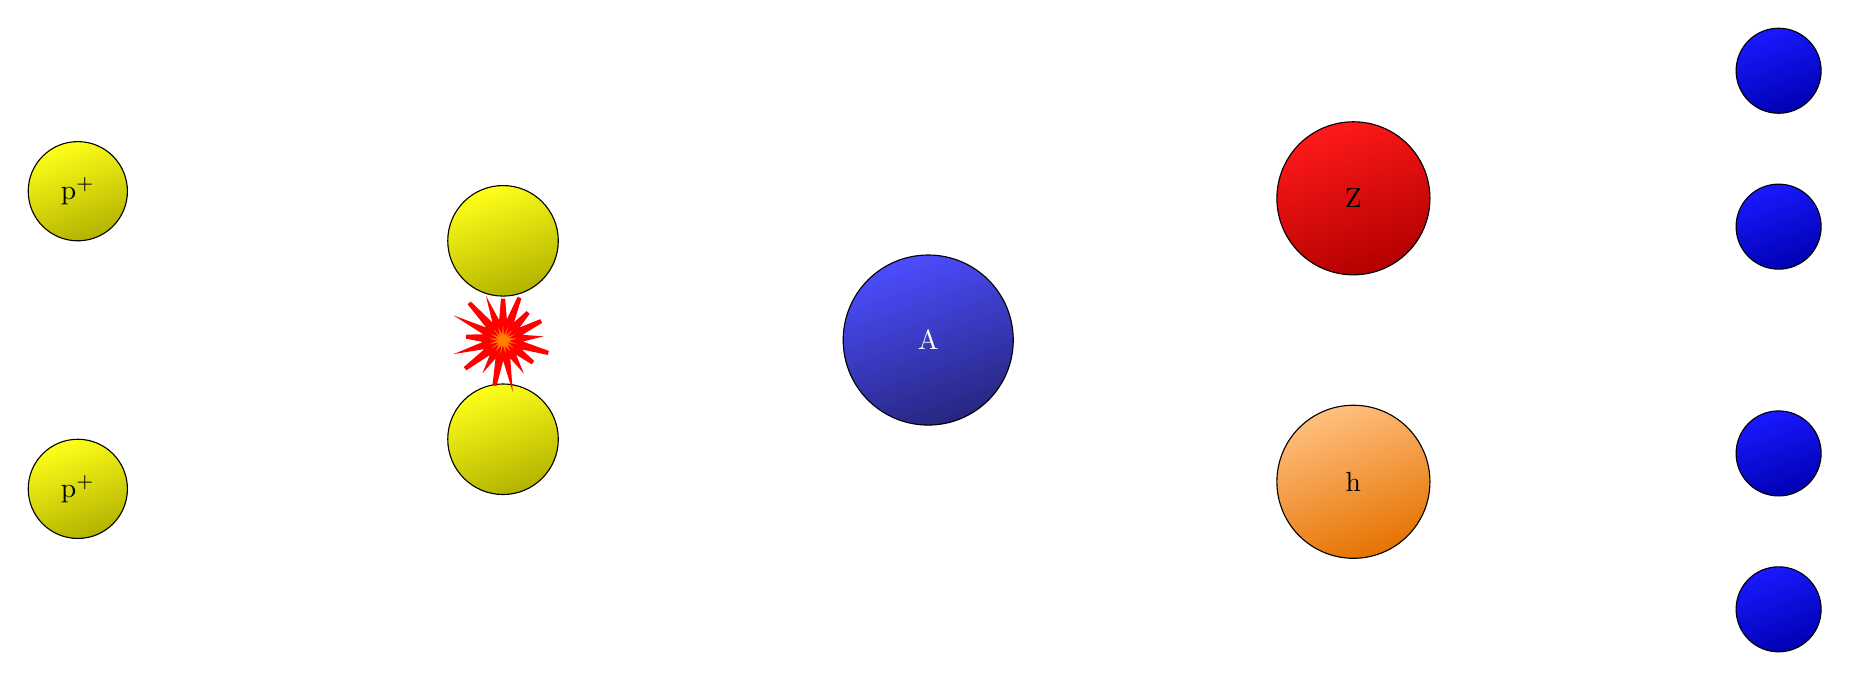
\begin{tikzpicture}[scale=0.9]
  
  \def\R{1.2}
  \def\Rp{0.7}
  
  \draw[proton] (0, 2.1) circle (\Rp) node {p$^+$};
  \draw[proton] (0,-2.1) circle (\Rp) node {p$^+$};
  
  \begin{scope}[shift={(6,0)}]
    \draw[proton] (0, 1.4) circle (0.65*\R); %node {p$^+$};
    \draw[proton] (0,-1.4) circle (0.65*\R); %node {p$^+$};
    \node[starburst, draw, minimum width=1 pt, minimum height=1 pt,red,fill=orange,line width=1.5pt] {};
  \end{scope}
  
  \begin{scope}[shift={(12,0)}]
    \draw[thin,draw=black,top color=blue!70!white,bottom color=blue!70!white!50!black,  shading angle=20]
      (0,0) circle (\R) node[white] {A};
  \end{scope}
  
  \begin{scope}[shift={(18,0)}]
    \draw[thin,draw=black,top color=red!90,   bottom color=red!70!black,   shading angle=20]
      (0, 2) circle (0.9*\R) node {Z};
    \draw[thin,draw=black,top color=orange!50,bottom color=orange!90!black,shading angle=20]
      (0,-2) circle (0.9*\R) node {h};
  \end{scope}
  
  \begin{scope}[shift={(24,0)}]
    \draw[thin,draw=black,top color=blue!90,  bottom color=blue!70!black,  shading angle=20]
      (0,-3.8) circle (0.5*\R);
    \draw[thin,draw=black,top color=blue!90,  bottom color=blue!70!black,  shading angle=20]
      (0,-1.6) circle (0.5*\R);
    \draw[thin,draw=black,top color=blue!90,  bottom color=blue!70!black,  shading angle=20]
      (0, 1.6) circle (0.5*\R);
    \draw[thin,draw=black,top color=blue!90,  bottom color=blue!70!black,  shading angle=20]
      (0, 3.8) circle (0.5*\R);
  \end{scope}
  
\end{tikzpicture}



\end{document}